\section{Cut Optimization \label{sec:Optim}}
All of the analyses calculate the predicted and observed number of tracks for numerous different sets of thresholds on the selection variables.
%The \muononly\ analysis evaluates thresholds with the \invbeta\ threshold ranging from 1.025 to 1.475 in steps of 0.025 and the $p_T$
%threshold ranging from 110 GeV to 450 GeV in steps of 30 GeV for a total of 240 different sets. The \tktof\ analysis
%varies the \invbeta\ threshold from 1.025 to 1.325 in steps of 0.025, the $p_T$ threshold from 50 GeV to 110 GeV in steps of 5 GeV up to 80 GeV
%and steps of 10 GeV after this, and the \ias\ threshold from 0.025 to 0.375 in steps of 0025 for a total of 2,101 different sets.
%%The \tkonly\ ,\fract, analysis has \pt\ thresholds from 50 GeV to 195 GeV and \ias, \iasp, thresholds from 0.025 to 0.425 for 480 different selection points. The
%The \tkonly\ analysis has \pt\ thresholds from 50 GeV to 195 GeV in steps of 5 GeV and \ias thresholds from 0.025 to 0.425 in steps of 0.025 for 480 different selection points.
%The \multi\ analysis has \invbeta\ thresholds from 1.025 to 1.45 in steps of 0.025 
%and \ias\ thresholds from 0.025 to 0.525 in steps of 0.025 giving a total of 260 different sets of selection thresholds.
Some of the sets of thresholds have only a small number of candidates in the control regions which are used to make the background prediction.
Low statistics in the control region can make the background prediction unreliable and potentially biased if signal candidates make up a large portion of the control region.
To prevent this, only thresholds that have at least 25 candidates in all control regions are considered. 
%For the \tktof\ and \tkonly\ analyses that use a mass cut it is additionally required that the control regions have at least a 

The number of predicted and observed events for a few sets of thresholds for the \muononly\ and \tktof\ analyses are shown in Figure~\ref{fig:PredPt230}. 
Similar plots are shown for the \tkonly\ and \multi\ analyses in Figure~\ref{fig:PredMF}.
The observed and predicted mass spectrum with loose thresholds is shown in Figure~\ref{fig:MassDistribution} for the
\tktof\ and \tkonly\ analyses.
%The number of predicted and observed events in the \multi\ and \fract\ analyses analysis for different selection points is shown in Fig.~\ref{fig:PredMF}.

\begin{figure}
\centering
  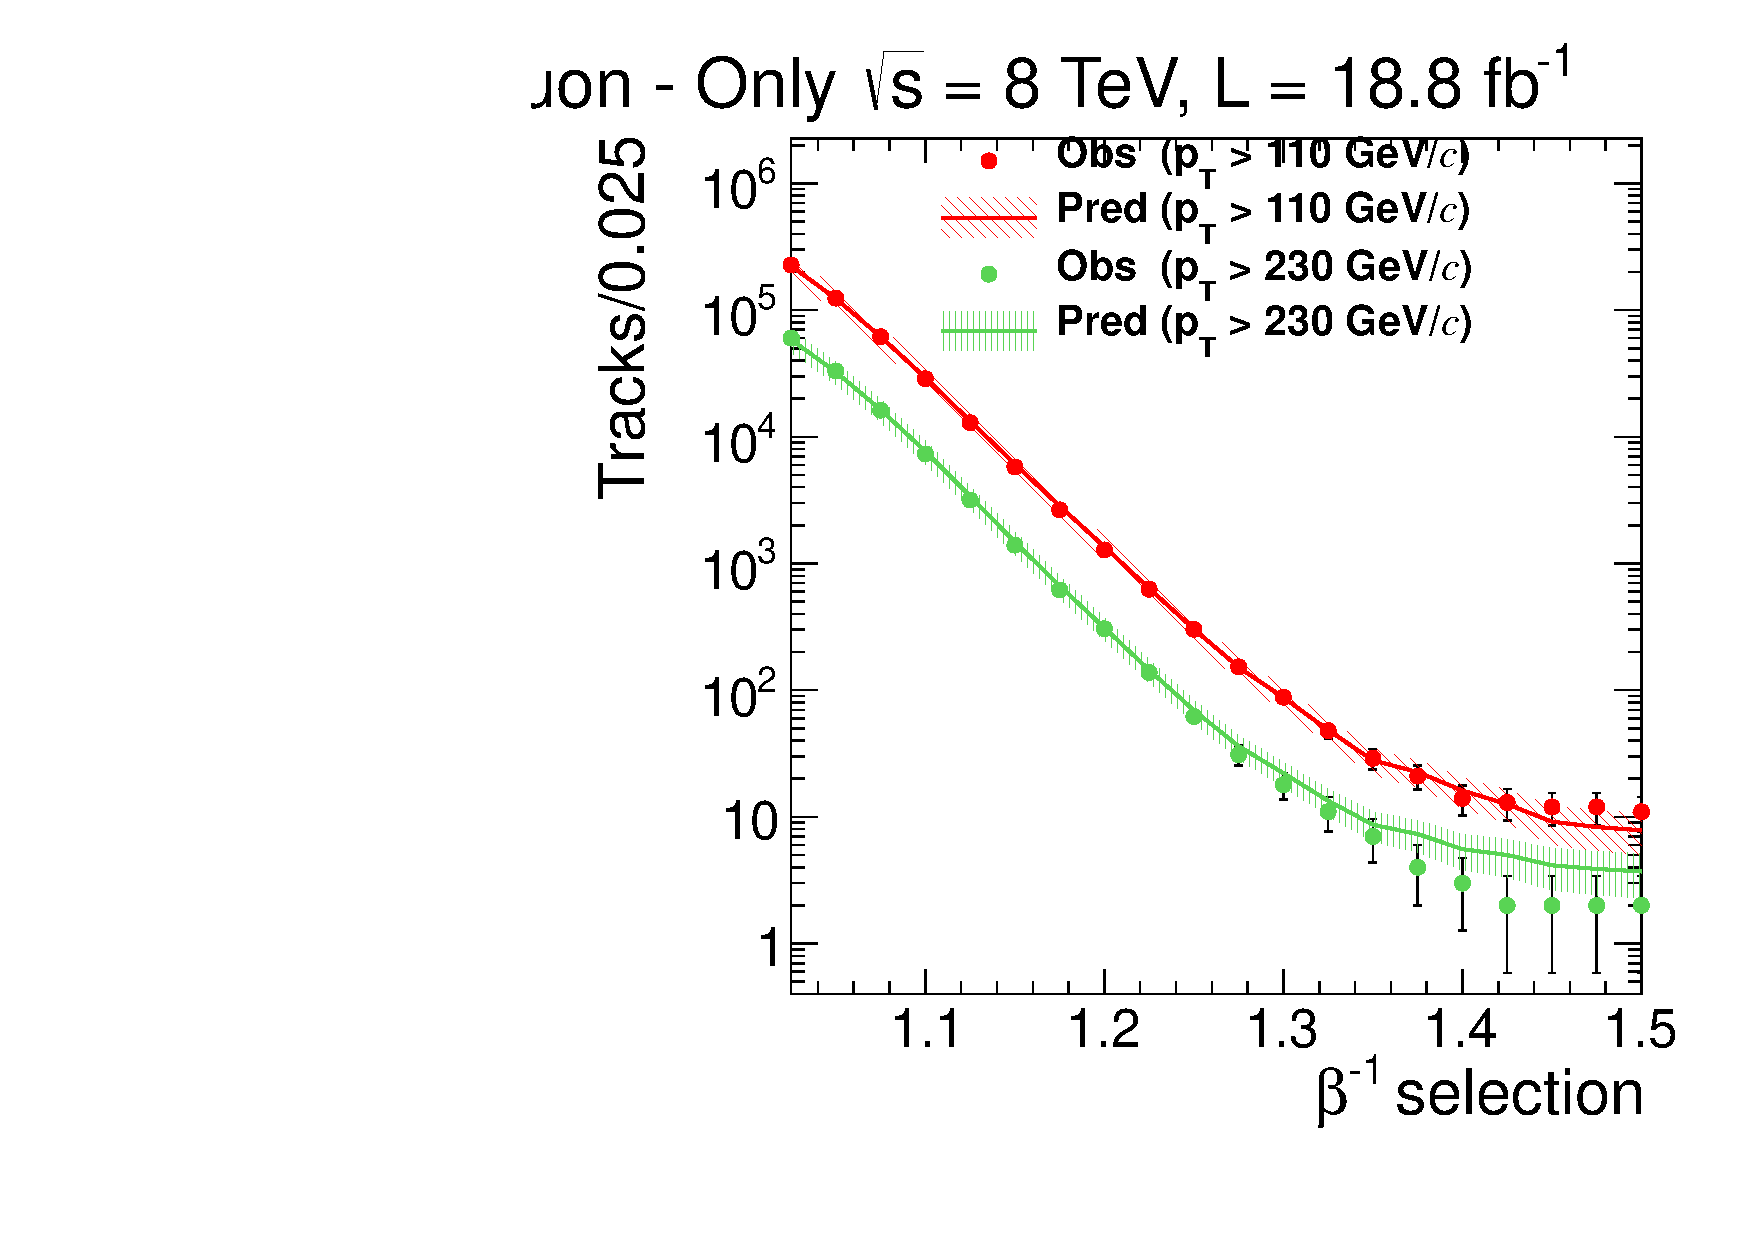
\includegraphics[clip=false, trim=0.0cm 0cm 0.0cm 0cm, width=0.48\textwidth]{figures/muonly/Prediction_Data8TeV_NPredVsNObs}
  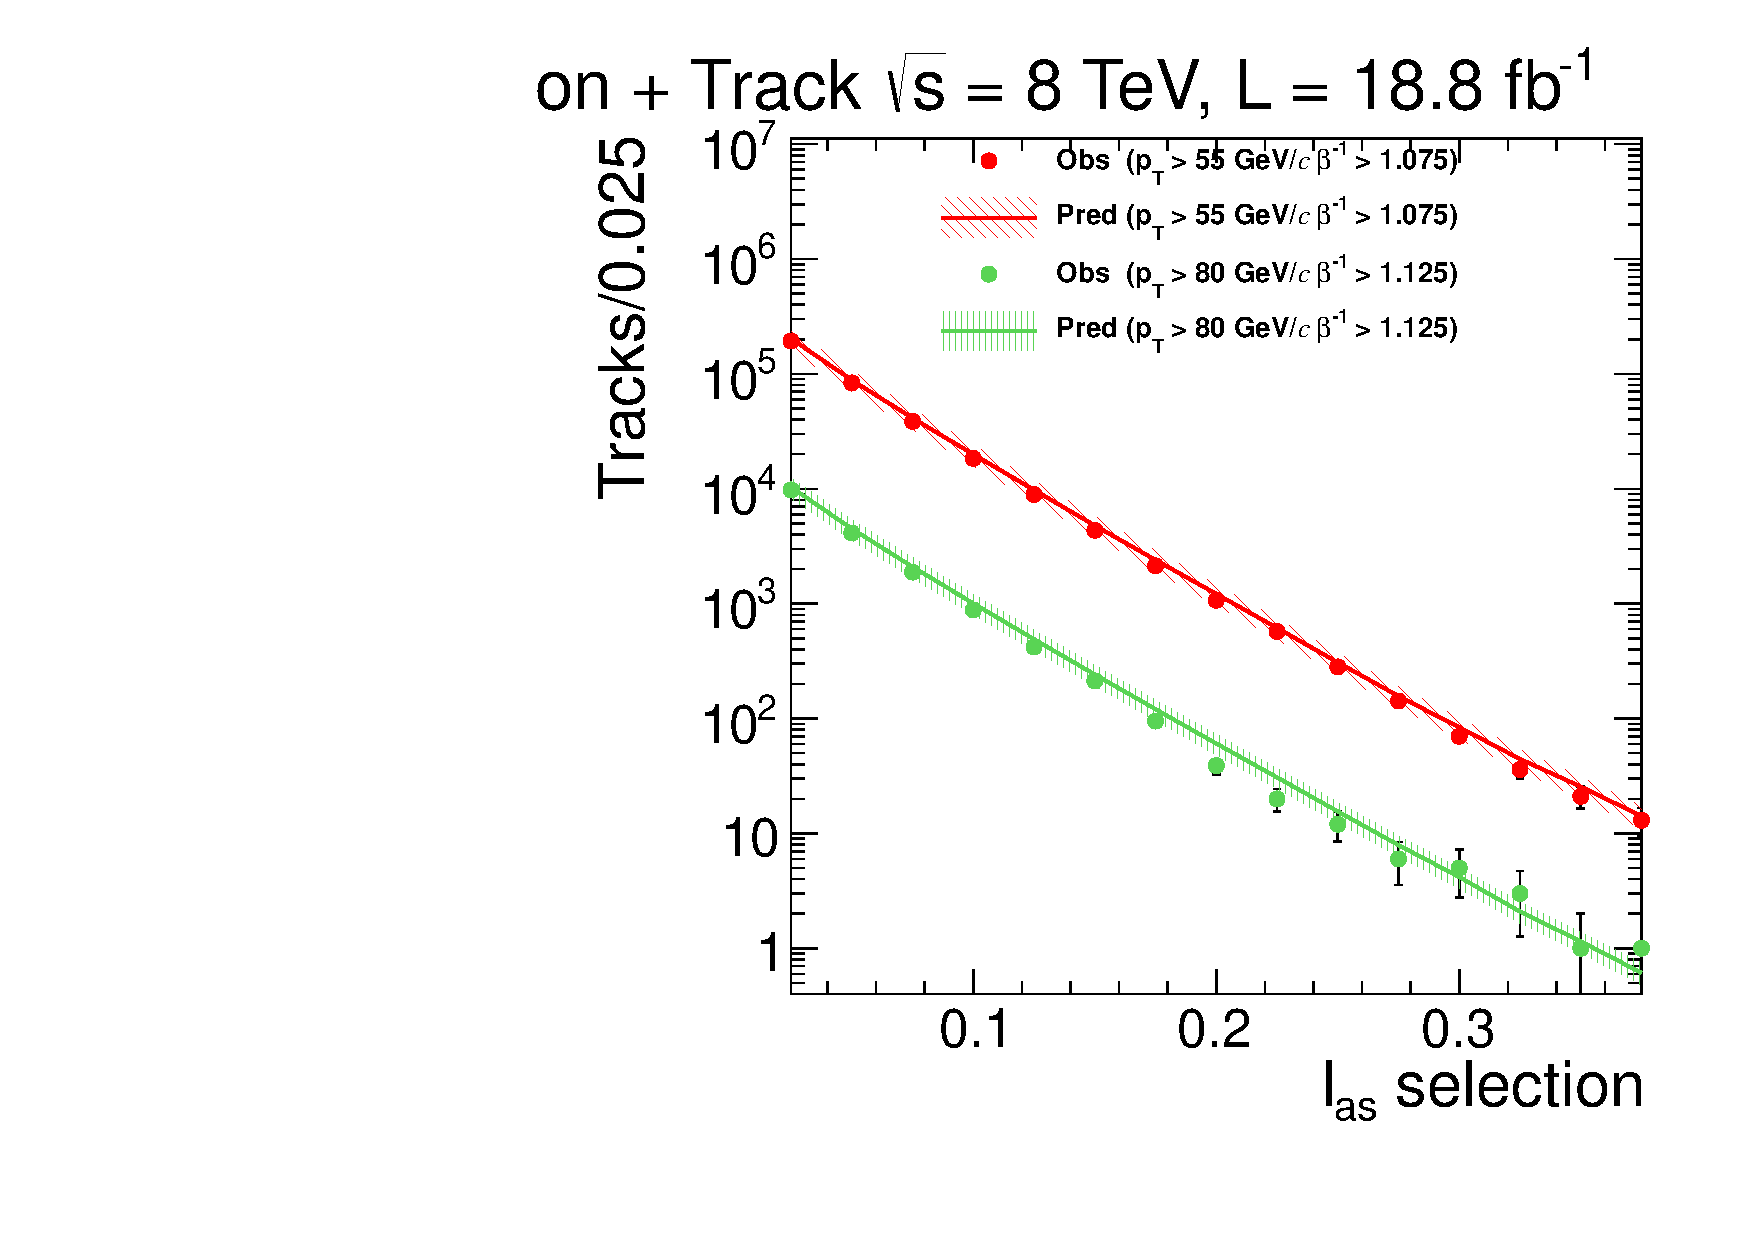
\includegraphics[clip=false, trim=0.0cm 0cm 0.0cm 0cm, width=0.48\textwidth]{figures/tkmu/Prediction_Data8TeV_NPredVsNObs}
  \caption[Number of predicted and observed events for two different thresholds in the \muononly\ and \tktof\ analyses.]
{Number of predicted and observed events for two different thresholds. 
Left: For the \muononly\ analysis. Threshold for \invbeta\ set by X-axis.
Right: For the \tktof\ analysis. The loose threshold is defined as \pt\ $>$ 55 GeV/$c$ and \invbeta\ $>$ 1.075.
The tight threshold is defined as \pt\ $>$ 80 GeV/$c$ and \invbeta\ $>$ 1.125.  Threshold for \ias\ set by X-axis.}
    \label{fig:PredPt230}
\end{figure}

\begin{figure}
\centering
  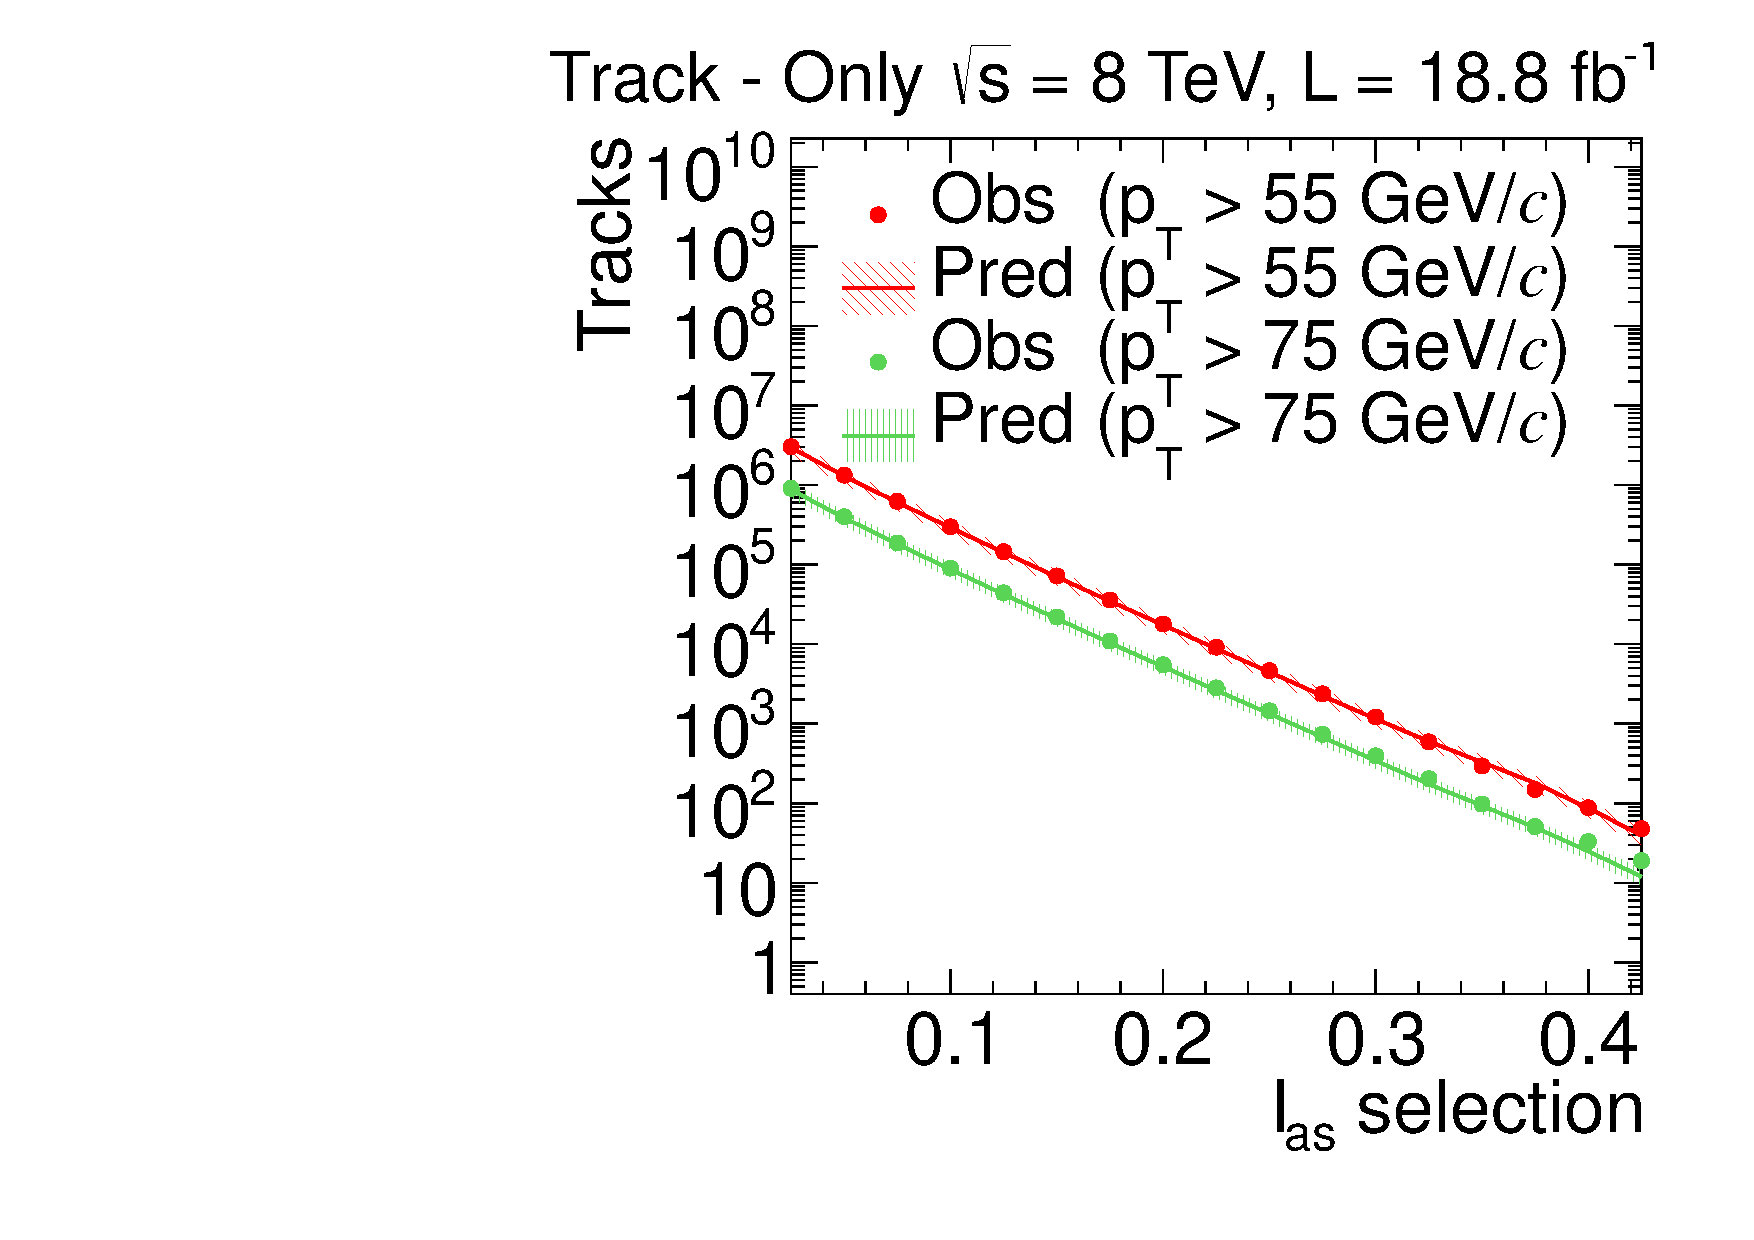
\includegraphics[clip=false, trim=0.0cm 0cm 0.0cm 0cm, width=0.48\textwidth]{figures/tkonly/Prediction_Data8TeV_NPredVsNObs}
  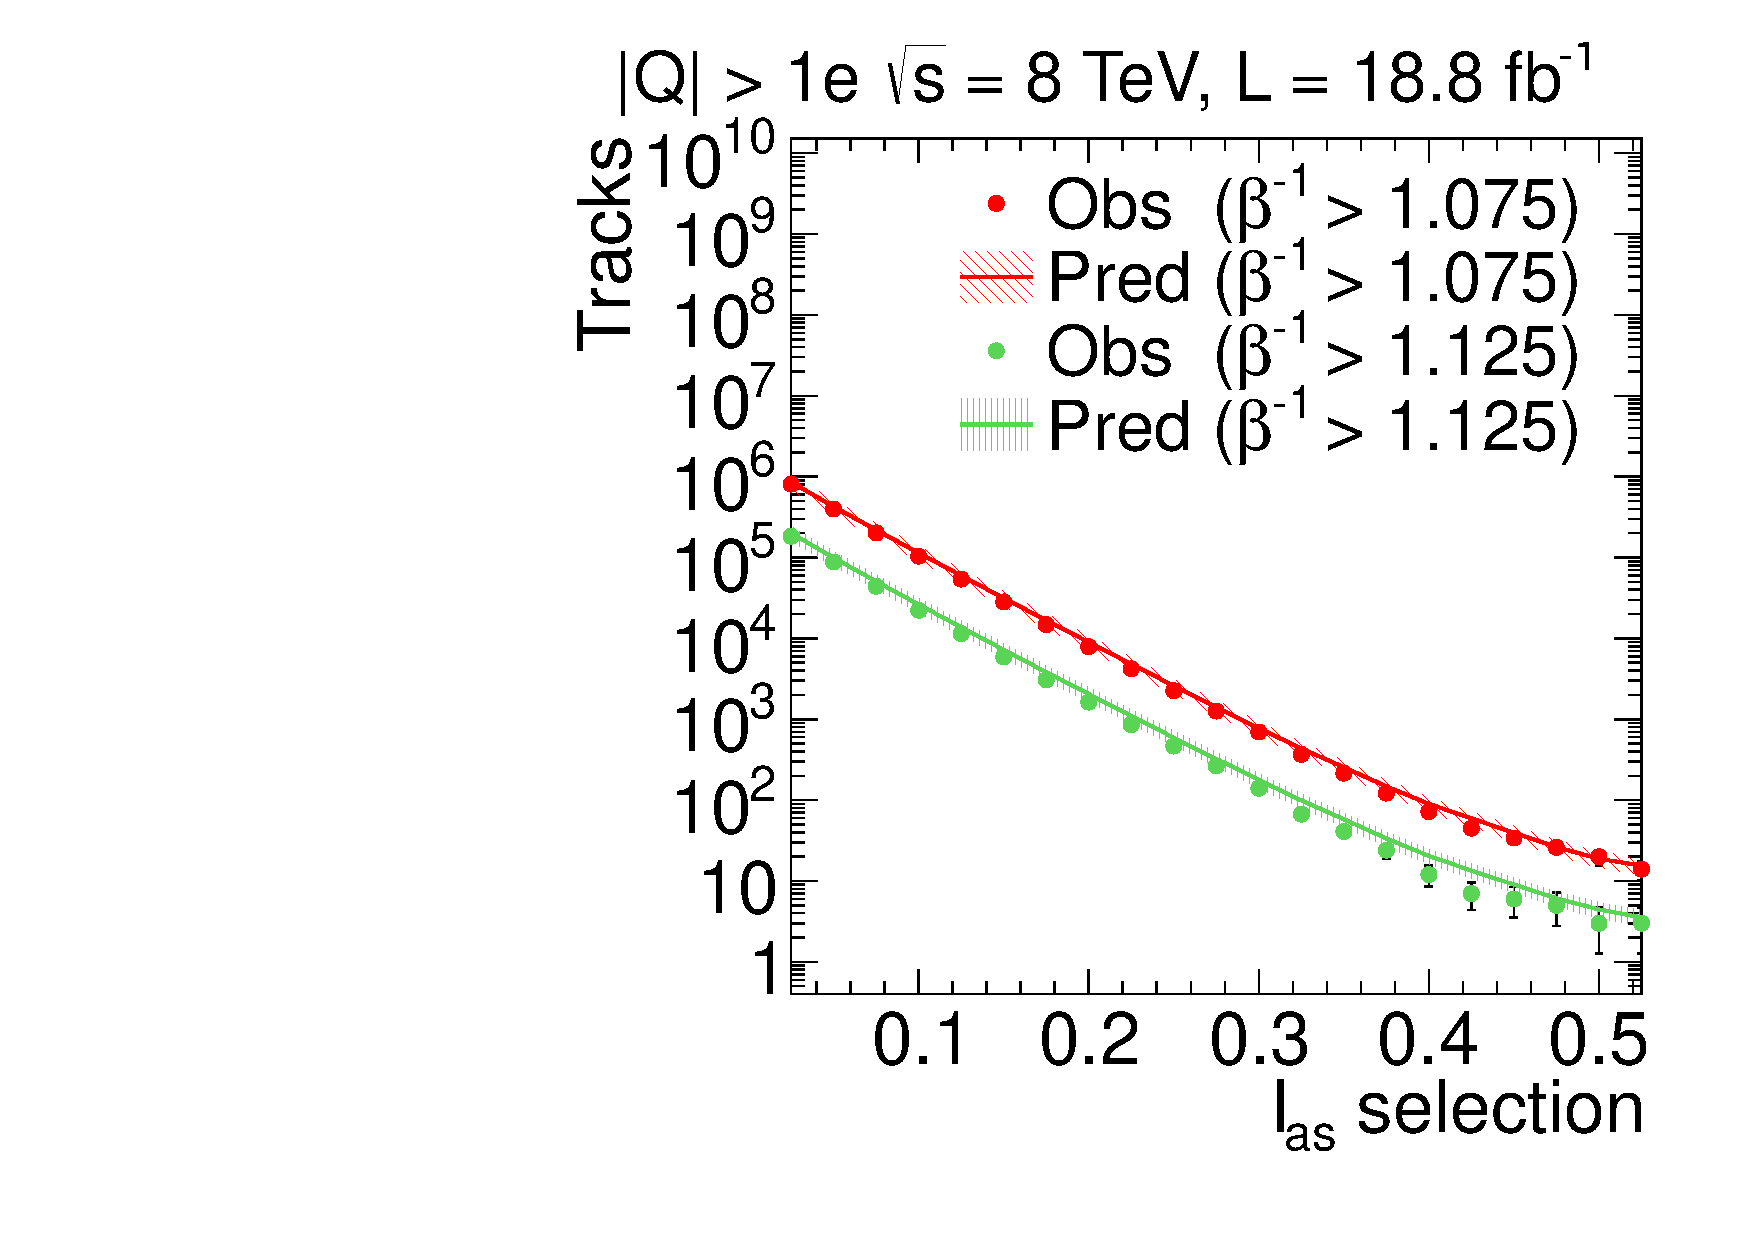
\includegraphics[clip=false, trim=0.0cm 0cm 0.0cm 0cm, width=0.48\textwidth]{figures/multi/Prediction_Data8TeV_NPredVsNObs}
  \caption[Number of predicted and observed events for two different thresholds in the \tkonly\ and \multi\ analyses.]
{Number of predicted and observed events for two different $p_T$ thresholds. Threshold for \ias\ set by X-axis.
Left: For the \tkonly\ analysis. Right: For the \multi\ analysis.}
    \label{fig:PredMF}
\end{figure}

\begin{figure}
 \begin{center}
  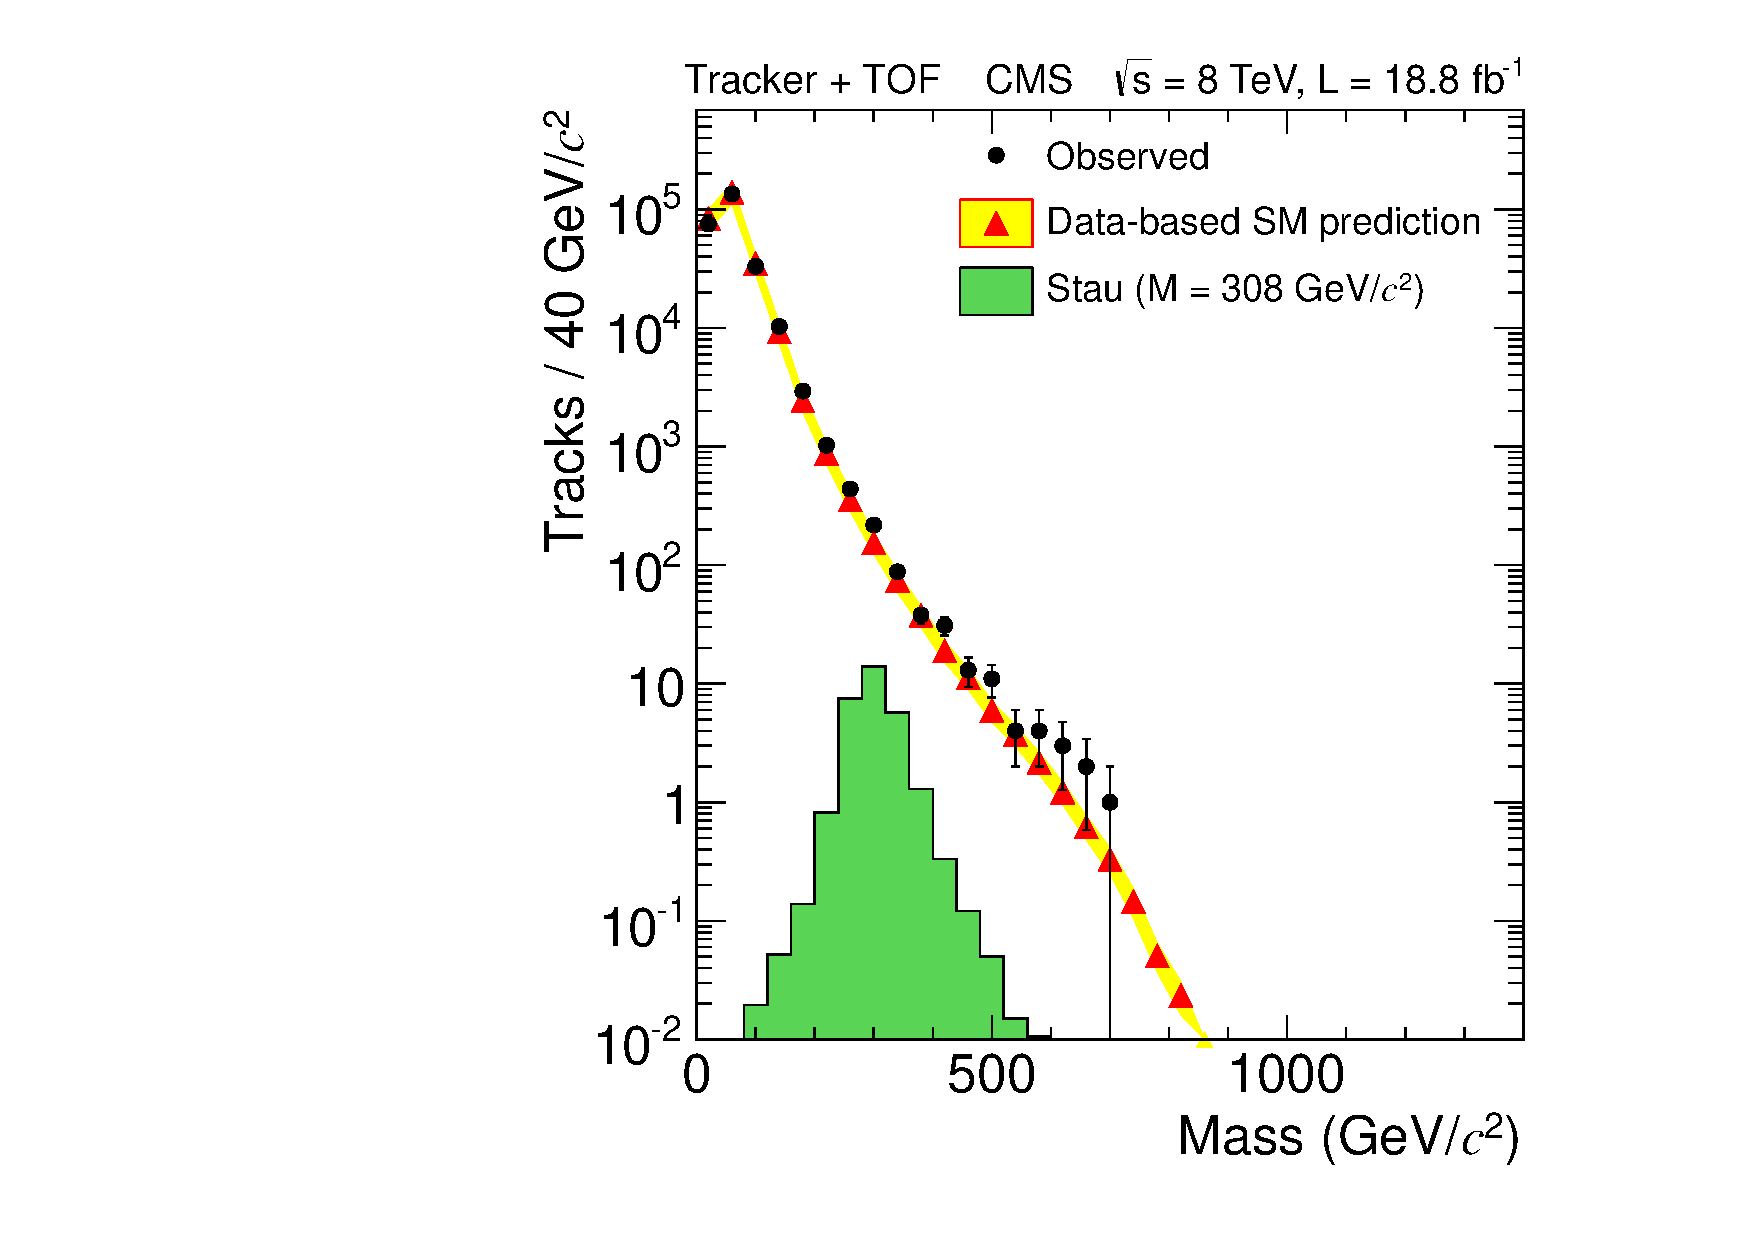
\includegraphics[clip=false, trim=0.0cm 0cm 0.0cm 0cm, width=0.48\textwidth]{figures/tkmu/RescaleNoRatio_Mass_8TeV_LooseNoSMMC}
  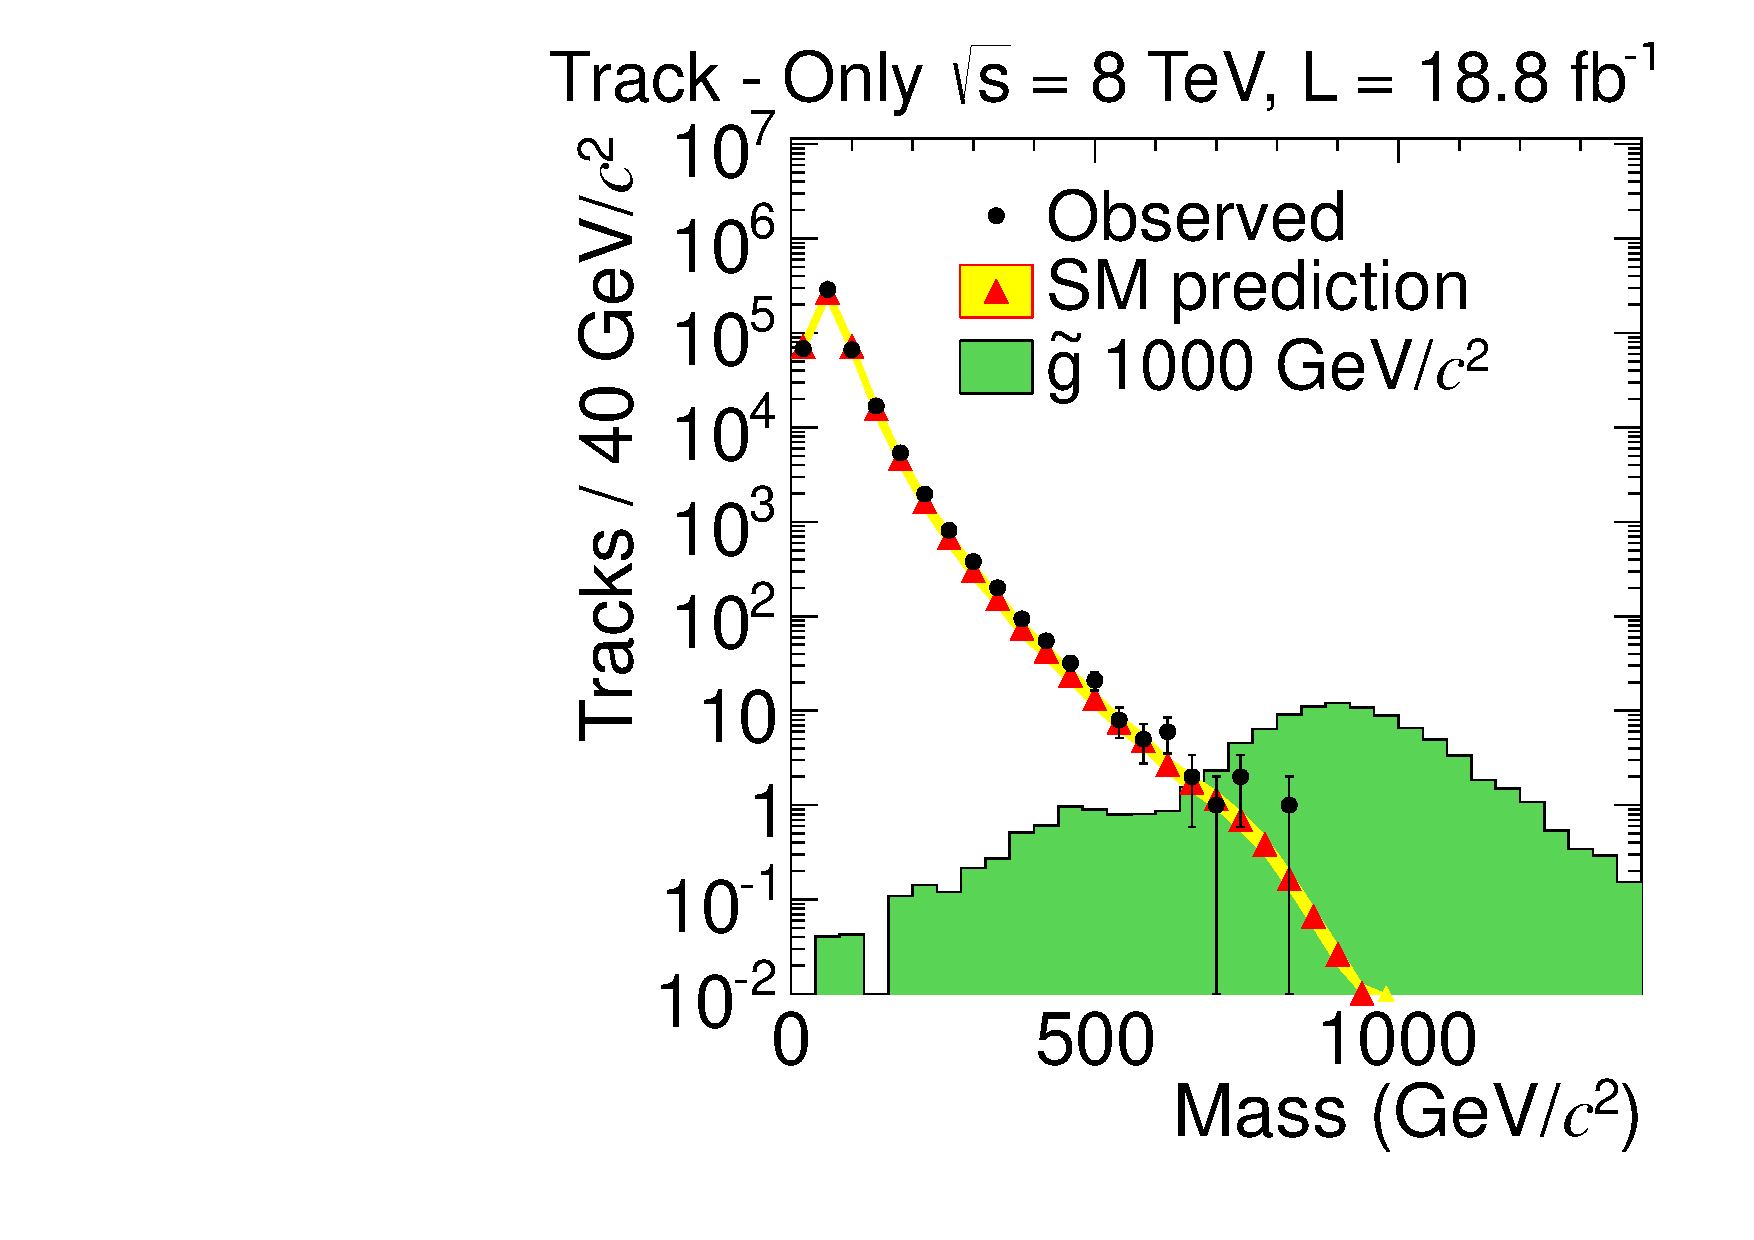
\includegraphics[clip=false, trim=0.0cm 0cm 0.0cm 0cm, width=0.48\textwidth]{figures/tkonly/RescaleNoRatio_Mass_8TeV_LooseNoSMMC}
 \end{center}
 \caption[Observed and predicted mass spectrum for candidates in the signal region with loose thresholds in the \tktof\ and \tkonly\ analyses.]
{Observed and predicted mass spectrum for candidates in the $D$ region with loose thresholds.
Left: For the \tktof\ analysis with thresholds of $p_T^{cut}>55$ GeV, $I_{as}>0.05$ and $1/\beta>1.05$.
Right: For the \tkonly\ analysis with thresholds of $p_T^{cut}>55$ GeV and $I_{as}>0.1$
The error bands are only statistical.}
\label{fig:MassDistribution}
\end{figure}

The thresholds on the selection variables are set trying to optimize two quantities, the expected reach and cross-section limit.
The two variables give the power of the analysis for two different hypotheses. Expected reach is concerned with the likelihood of finding a signal if it does exist while the
expected limit is concerned with excluding the signal if it does not exist.

When optimizing the expected reach it is necessary to be careful not to optimize to
a region with very small predicted background at the expense of signal efficiency. 
The reason is that for very small predicted background it is possible to have a five sigma
significance with only one or two observed events. For example, one observed event will give a five sigma significance for a predicted background of $2.87\times10^{-7}$.
However, a single event is normally not enough to claim discovery of new physics.
To protect against this, the definition of the expected reach is modified to be at least as large as
the cross-section which is expected to give at least five events, as recommended by the CMS statistics committee.

Most of the time, the two variables agree which of two sets of thresholds is better however in some
conditions the variables will disagree. One such case is analyses that have little predicted background and high efficiency for the signal to pass the thresholds on the
selection variables. This is the case for high mass samples in the \tktof\  and \tkonly\ analyses.

Once the expected cross-section limit falls below the point where more than 50\% of the time zero events would be observed in the background only hypothesis,
the expected cross-section limit no longer improves
by decreasing the expected background. Any loss of efficiency caused by raising the threshold on the selection variables will cause the expected cross-section limit to be optimized
at this crossover point. The crossover occurs at approximately 0.6 predicted events with the uncertainties used in the analyses. 

The expected reach continues to improve by making the predicted background smaller until a five sigma significance would be found with fewer than five events. At this
point the requirement that at least five events be found for a discovery sets the expected reach.
This occurs at approximately 0.1 predicted events. 

Thus how low the predicted background can be is set differently when optimizing for one versus the other.
When the optimization for the best expected reach is used for these cases, the
effect on the expected cross-section limit is usually small as the signal efficiency does not decrease much when raising the thresholds. However
when the optimization from the expected limit is used, the expected reach can get noticeably worse as more events are needed to claim a discovery.
% as twice? as many events are needed. This can be seen in
%Figs.~\ref{fig:ReachLimitRatio} and~\ref{fig:LimitReachRatio} which show the ratio of the expected cross-section limit when optimizing for the best best expected reach
%relative to when optimizing for the best expected cross-section limit and the ratio of the expected reach when optimizing for the best expected cross-section limit
%relative to when optimizing for the best expected reach. 
For this reason, combined with the fact that the main goal of these analyses is to discover new physics, priority
is given to the expected reach when trying to optimize the threshold values.

%\begin{figure}
%\begin{center}
%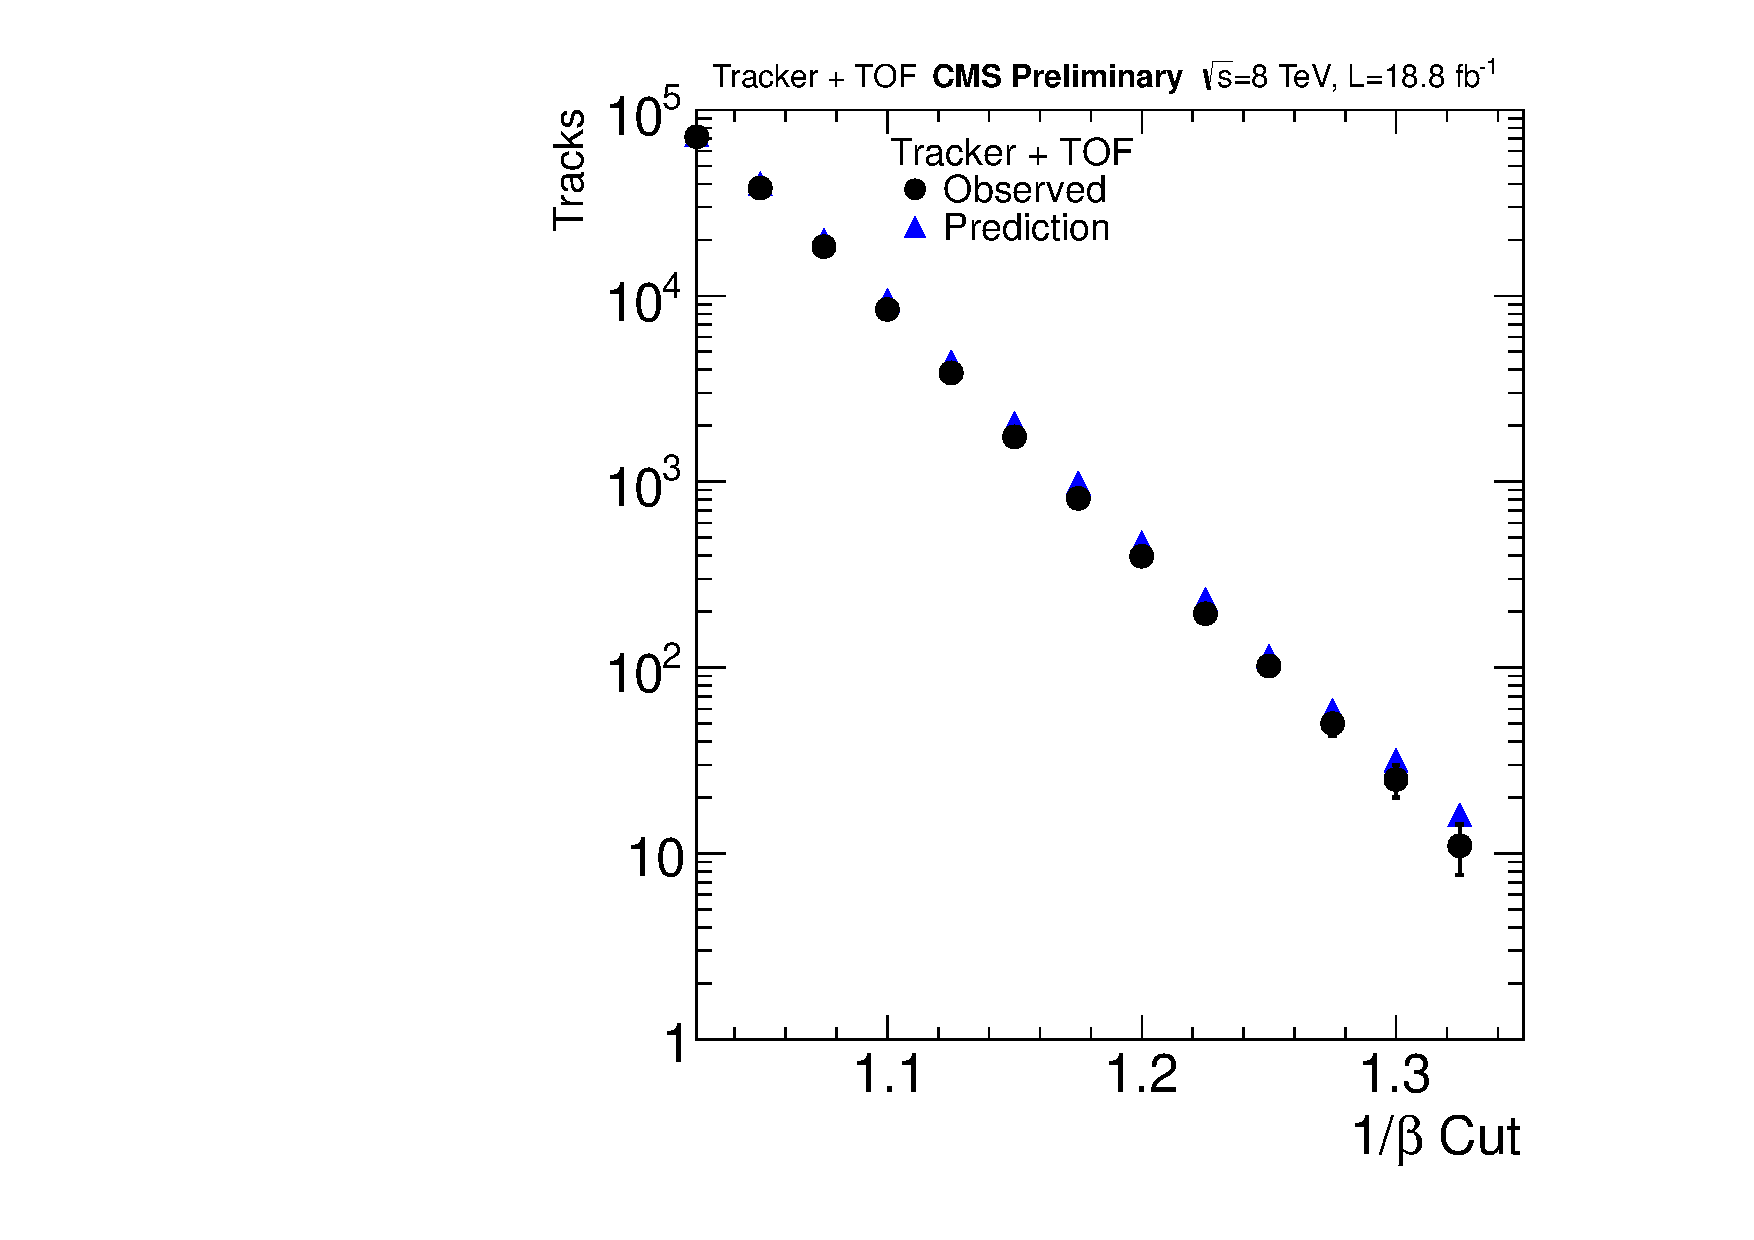
\includegraphics[clip=true, trim=0.0cm 0cm 3.0cm 0cm, width=0.44\textwidth]{figures/tkmu/Pred_I010_Pt55_Data8TeV}
%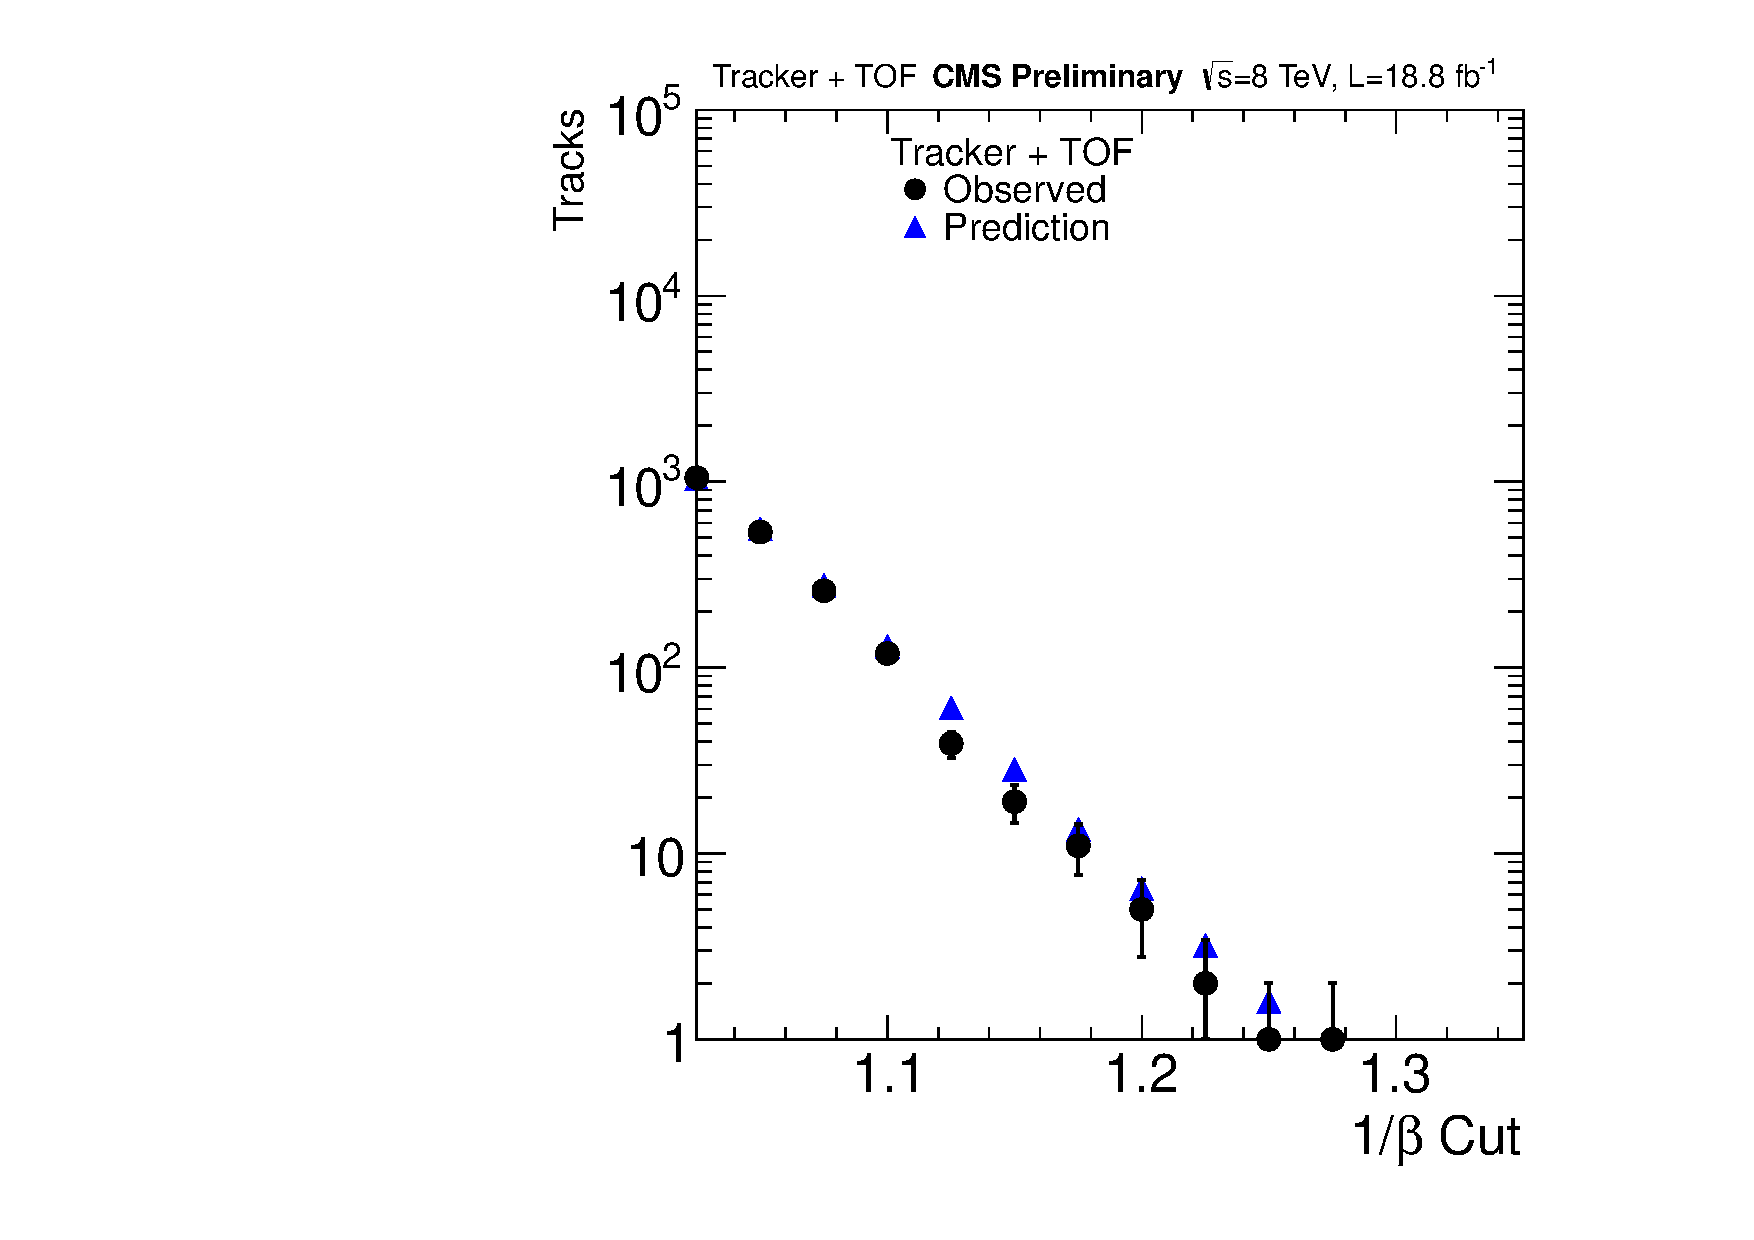
\includegraphics[clip=true, trim=0.0cm 0cm 3.0cm 0cm, width=0.44\textwidth]{figures/tkmu/Pred_I020_Pt80_Data8TeV}
%\caption{Number of observed and predicted events and their statistical error in the $D$ region for $p_T>55, I_{as}>0.1$ (left)
%and $p_T>80, I_{as}>0.2$ (right). Threshold on $1/\beta$ defined by the x-axis
%\label{fig:ReachLimitRatio}}
%\end{center}
%\end{figure}

%\begin{figure}
%\begin{center}
%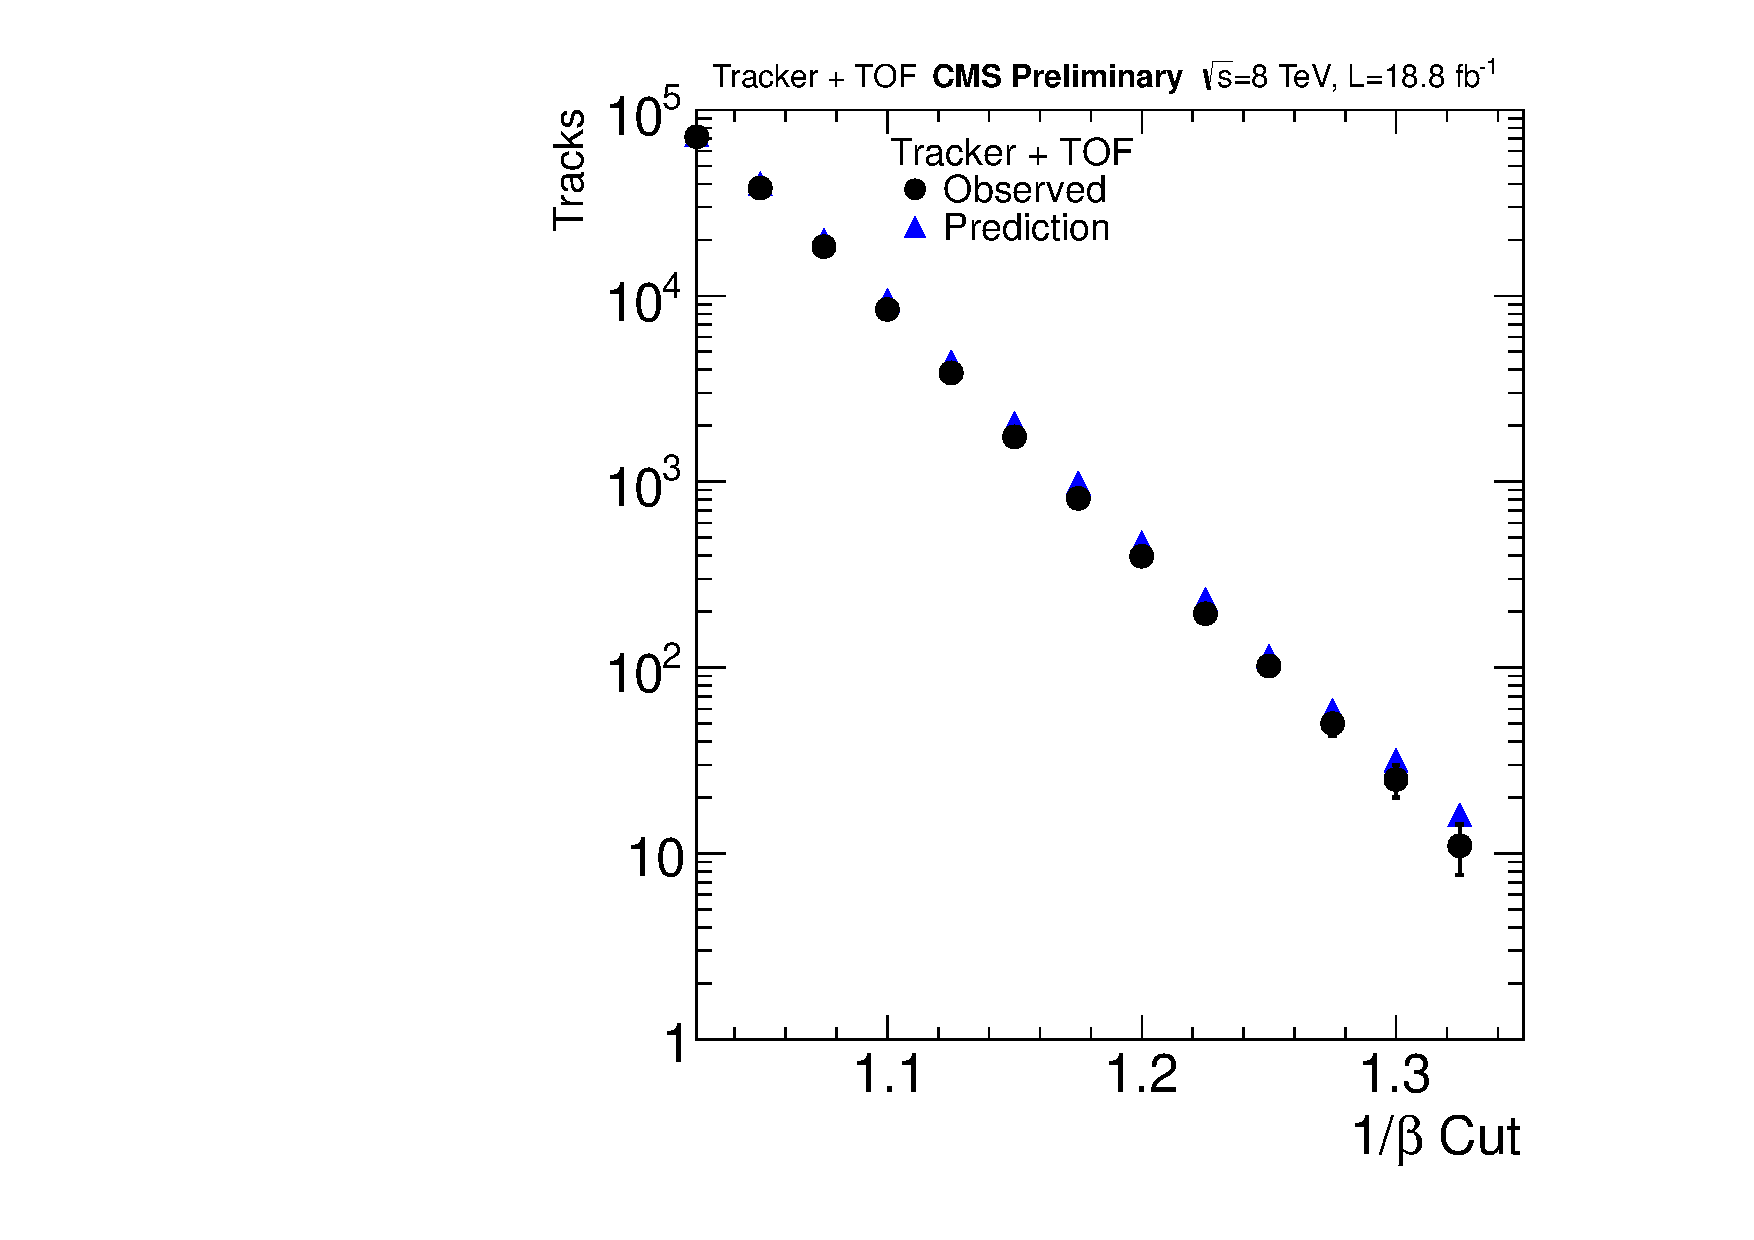
\includegraphics[clip=true, trim=0.0cm 0cm 3.0cm 0cm, width=0.44\textwidth]{figures/tkmu/Pred_I010_Pt55_Data8TeV}
%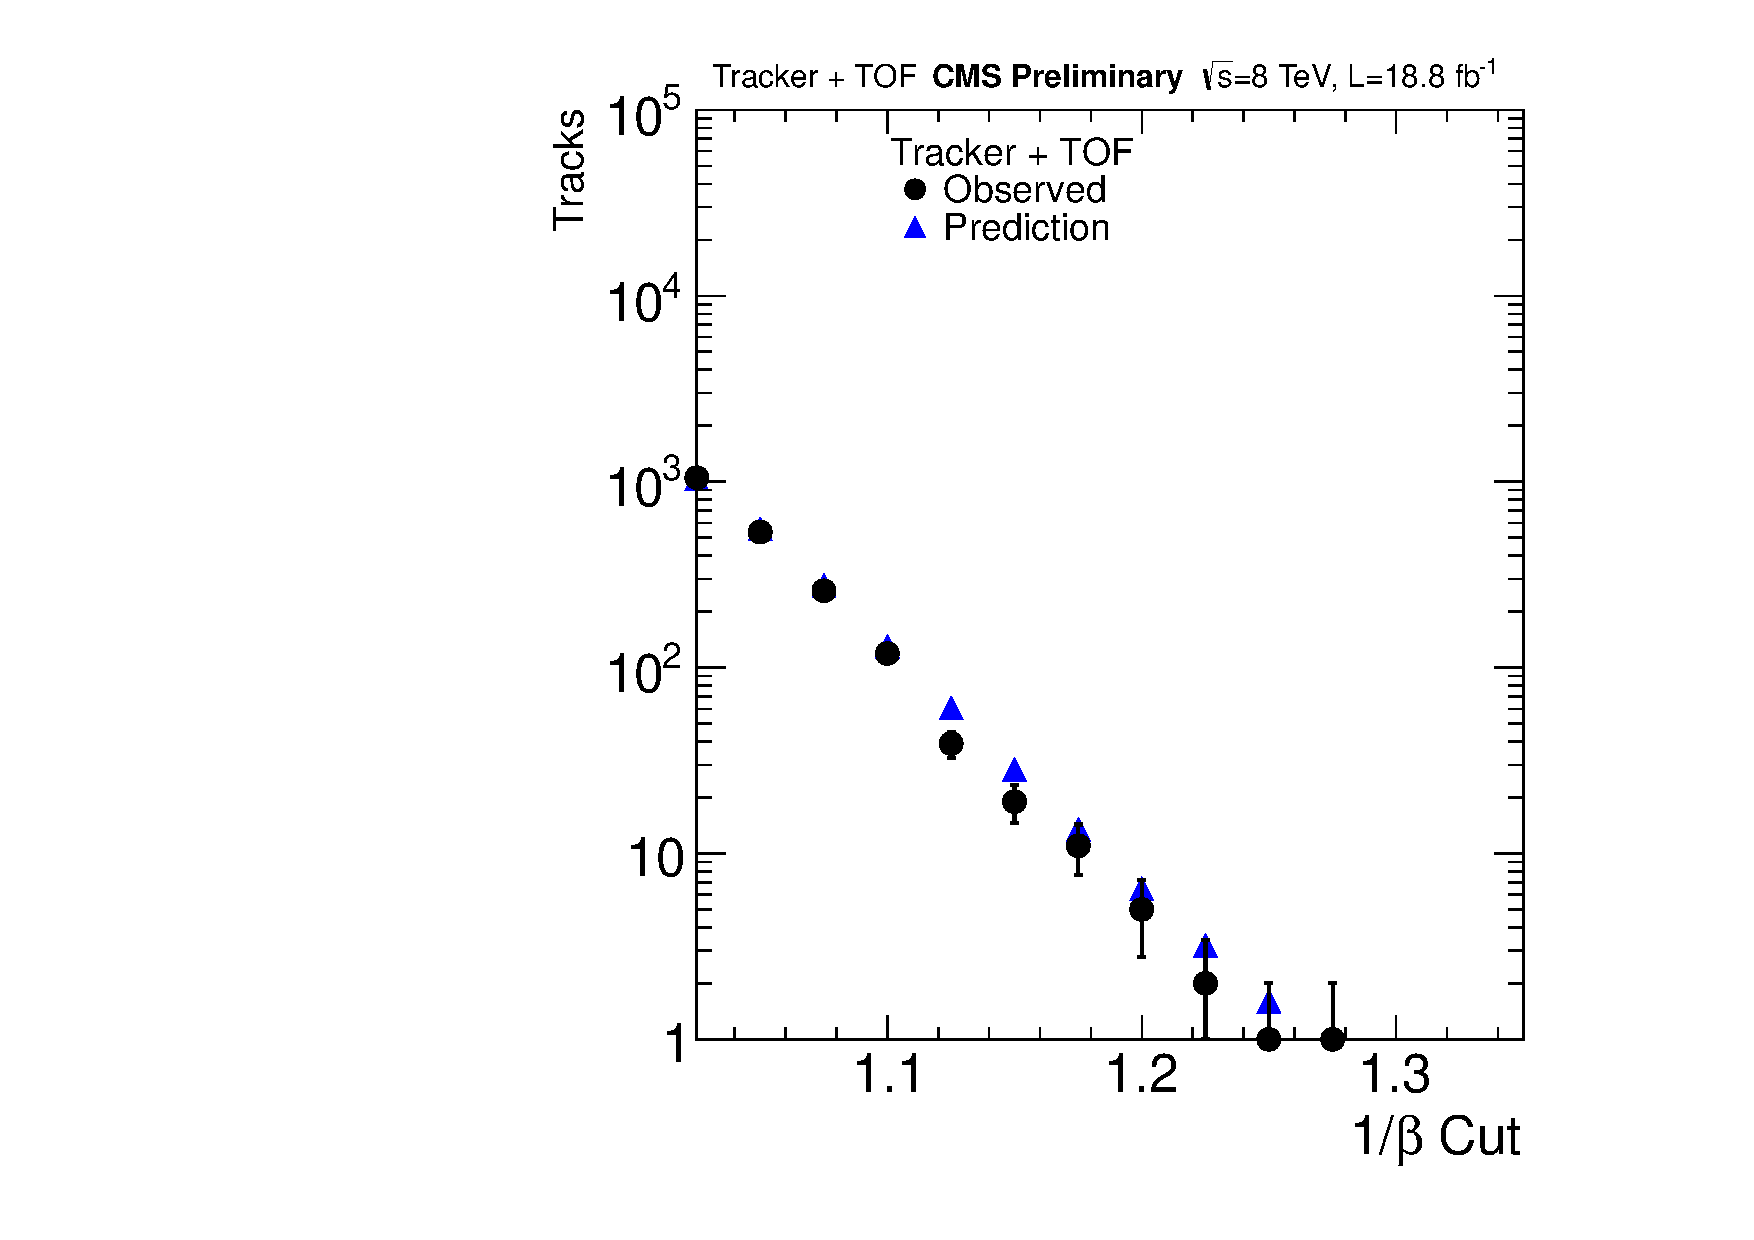
\includegraphics[clip=true, trim=0.0cm 0cm 3.0cm 0cm, width=0.44\textwidth]{figures/tkmu/Pred_I020_Pt80_Data8TeV}
%\caption{Number of observed and predicted events and their statistical error in the $D$ region for $p_T>55, I_{as}>0.1$ (left)
%and $p_T>80, I_{as}>0.2$ (right). Threshold on $1/\beta$ defined by the x-axis
%\label{fig:LimitReachRatio}}
%\end{center}
%\end{figure}

The thresholds are optimized in a two step process. First the set of thresholds which give the best expected reach for each mass/model point is determined. However, this leads
to numerous different selections being used which are often very similar and give about the same discriminating power. This is troublesome for two reasons. 

The first is that using multiple different selections increases the risk of a statistical fluctuation of the background causing a spurious signal. 
To account for this a correction
must be applied to the obtained local significance such that the value is correctly set to the probability of finding the signal in any of the used sets of thresholds. This
means that the global expected reach could be improved by using fewer sets of thresholds even if it comes with the price of making the local expected reach worse.

The second reason is that the analysis becomes much more difficult to understand as there are multiple different sets of thresholds being used as well as multiple predicted and 
observed events. This complexity brings with it little additional gain in the expected reach or cross section limit and unnecessary complexity is not something that
is desired in an analysis. No matter how robust an analysis is, if it can not be 
understood by others then it can not have an impact on the scientific community at large.

For these reasons a second step is taken attempting to make the thresholds the same for the various mass/model points. If the harm to mass/model points in having the
same thresholds is too large then using more than one set of thresholds is possible. 
However this was found not to be necessary and a single cut value is used in all analyses. 

The final thresholds used as well as the number of
observed and predicted events is shown in Table~\ref{tab:finalsel}. 
The number of observed events is found to be consistent with the expected background.
The largest excess for any of the selections shown in the table is 1.0 sigma in the \tkonly\ analysis with no mass cut.
The predicted and observed mass distributions for the \tkonly\ and \tktof\ analyses
with the final thresholds are shown in Figure~\ref{fig:TightMassDistribution}. 

\begin{table}
 \caption[Results of the final selections for predicted background and
   observed number of events in all of the analyses.]
{Results of the final selections for predicted background and
   observed number of events. Results for representative mass cuts are given for the \tkonly\ and \tktof\ analyses. Uncertainties are statistical and systematic.
   \label{tab:finalsel}}
 \begin{center}
 \begin{tabular}{|l|c|c|c|c|cc|} \hline
%                        & \multicolumn{4}{c|}{~}                                         & \multicolumn{2}{c|}{Numbers of events} \\
                        & \multicolumn{4}{c|}{\textbf{Selection criteria}}               & \multicolumn{2}{c|}{Number of events}  \\ \hline
                        & $p_T $                  & \multirow{2}{*}{\ias}      & \multirow{2}{*}{\invbeta}  & Mass      & \multirow{2}{*}{Pred.} & \multirow{2}{*}{Obs.} \\
                        & ($GeV/c$)               &                            &                            & $GeV/c^2$ &                &                    \\ \hline
\muononly\              & $> 230$                 &  -                         & $> 1.40$                   &    -      & $5.6\pm2.9$    & $3$  \\ \hline
\multirow{4}{*}{\tktof} & \multirow{4}{*}{$> 70$} & \multirow{4}{*}{$> 0.125$} & \multirow{4}{*}{$> 1.225$} & $>   0$   & $43.5\pm8.7$   & $42$ \\
                        &                         &                            &                            & $> 100$   & $5.6\pm1.1$    & $7$  \\
                        &                         &                            &                            & $> 200$   & $0.56\pm0.11$  & $0$  \\
                        &                         &                            &                            & $> 300$   & $0.090\pm0.02$ & $0$  \\ \hline
\multirow{4}{*}{\tkonly}& \multirow{4}{*}{$> 70$} & \multirow{4}{*}{$> 0.4$}   & \multirow{4}{*}{$-$}       & $>   0$   & $32.5\pm6.5$   & $41$ \\
                        &                         &                            &                            & $> 100$   & $26.0\pm5.2$   & $29$ \\
                        &                         &                            &                            & $> 200$   & $3.1\pm0.6$    & $3$  \\
                        &                         &                            &                            & $> 300$   & $0.55\pm0.11$  & $1$  \\
                        &                         &                            &                            & $> 400$   & $0.15\pm0.03$  & $0$ \\ \hline
$|Q|>1e$                &           $-$           &       $> 0.500$            &        $> 1.200 $          &    $-$    & $0.52\pm 0.11$ & $1$ \\ \hline
%$|Q|<1e$                & $> 125$                 & $>0.275$                   &            $-$             &    $-$    & $0.99\pm0.24$  & $0$ \\ \hline

 \end{tabular}
 \end{center}
\end{table}

\begin{figure}
 \begin{center}
  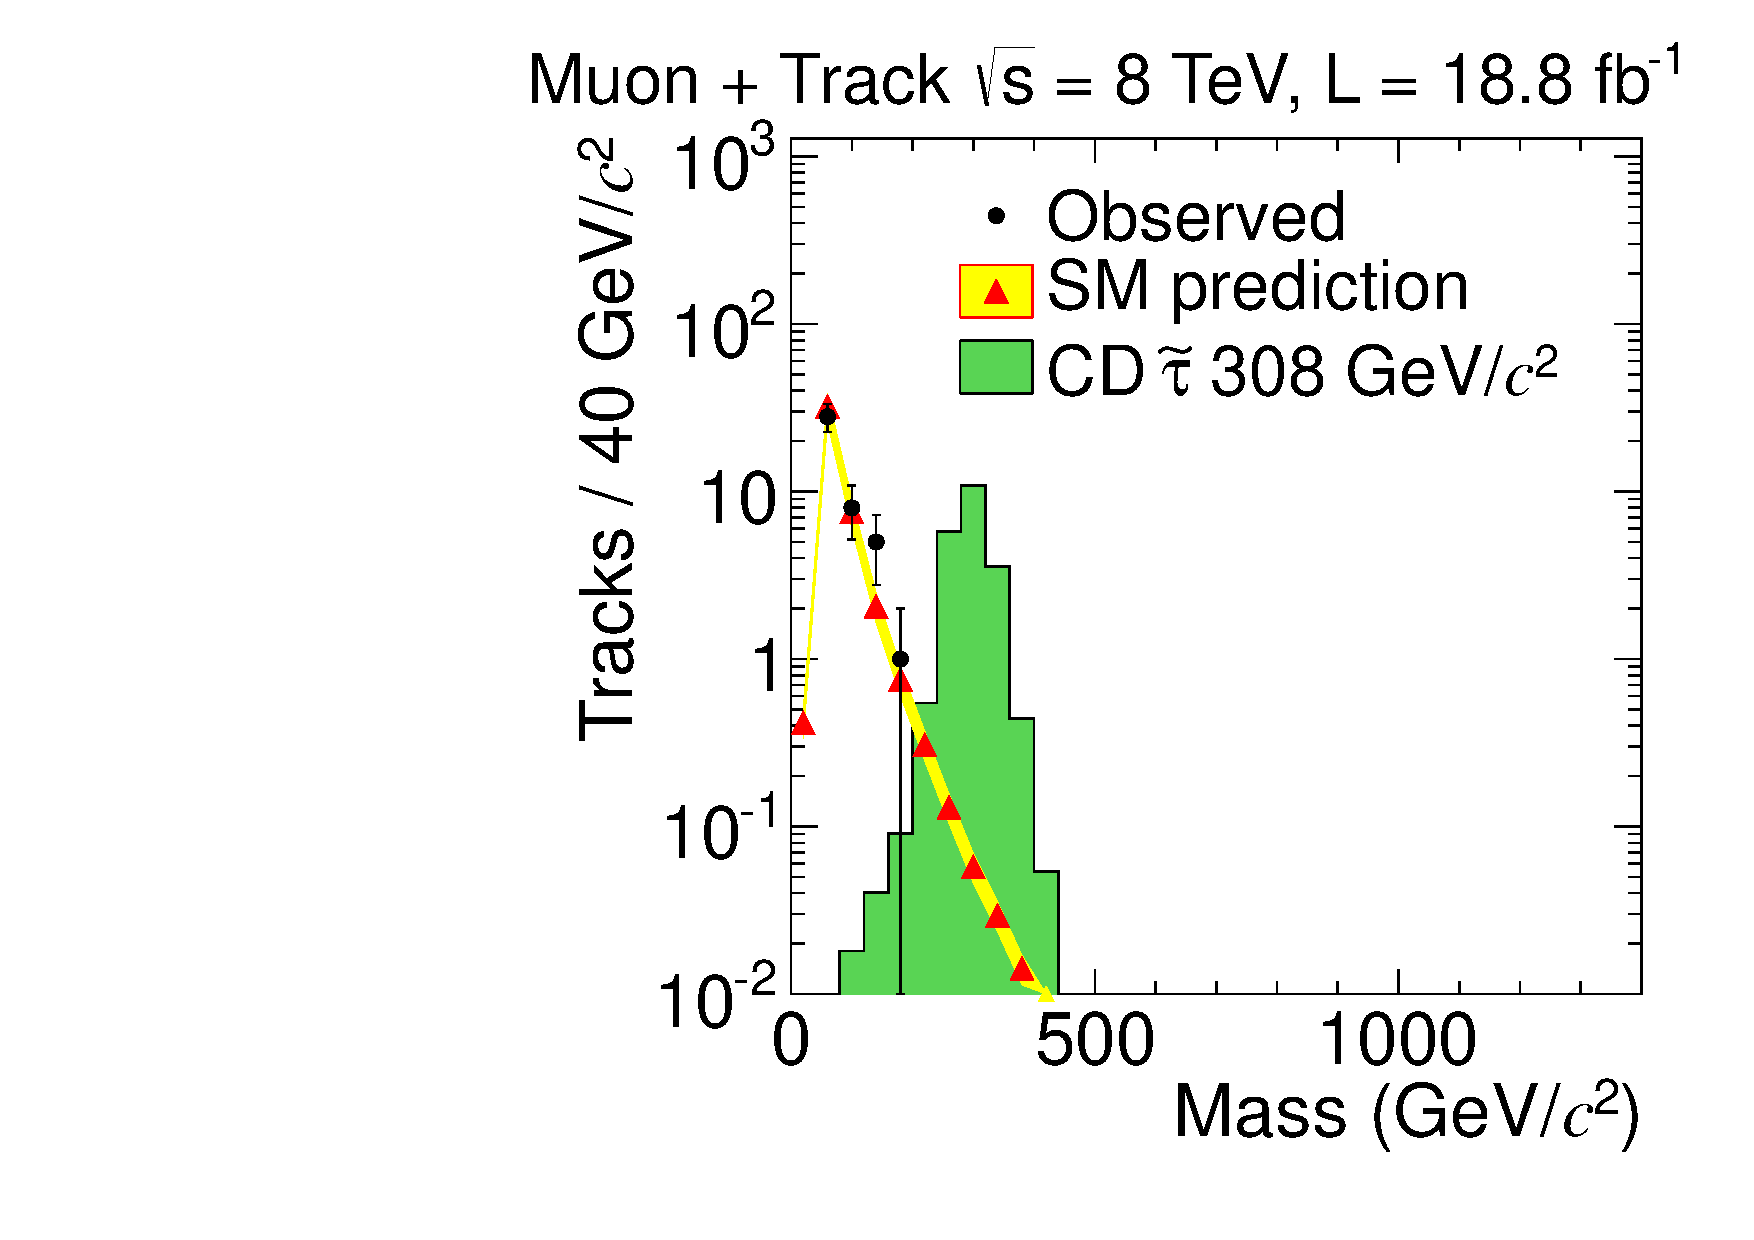
\includegraphics[clip=false, trim=0.0cm 0cm 0.0cm 0cm, width=0.48\textwidth]{figures/tkmu/RescaleNoRatio_Mass_8TeV_TightNoSMMC}
  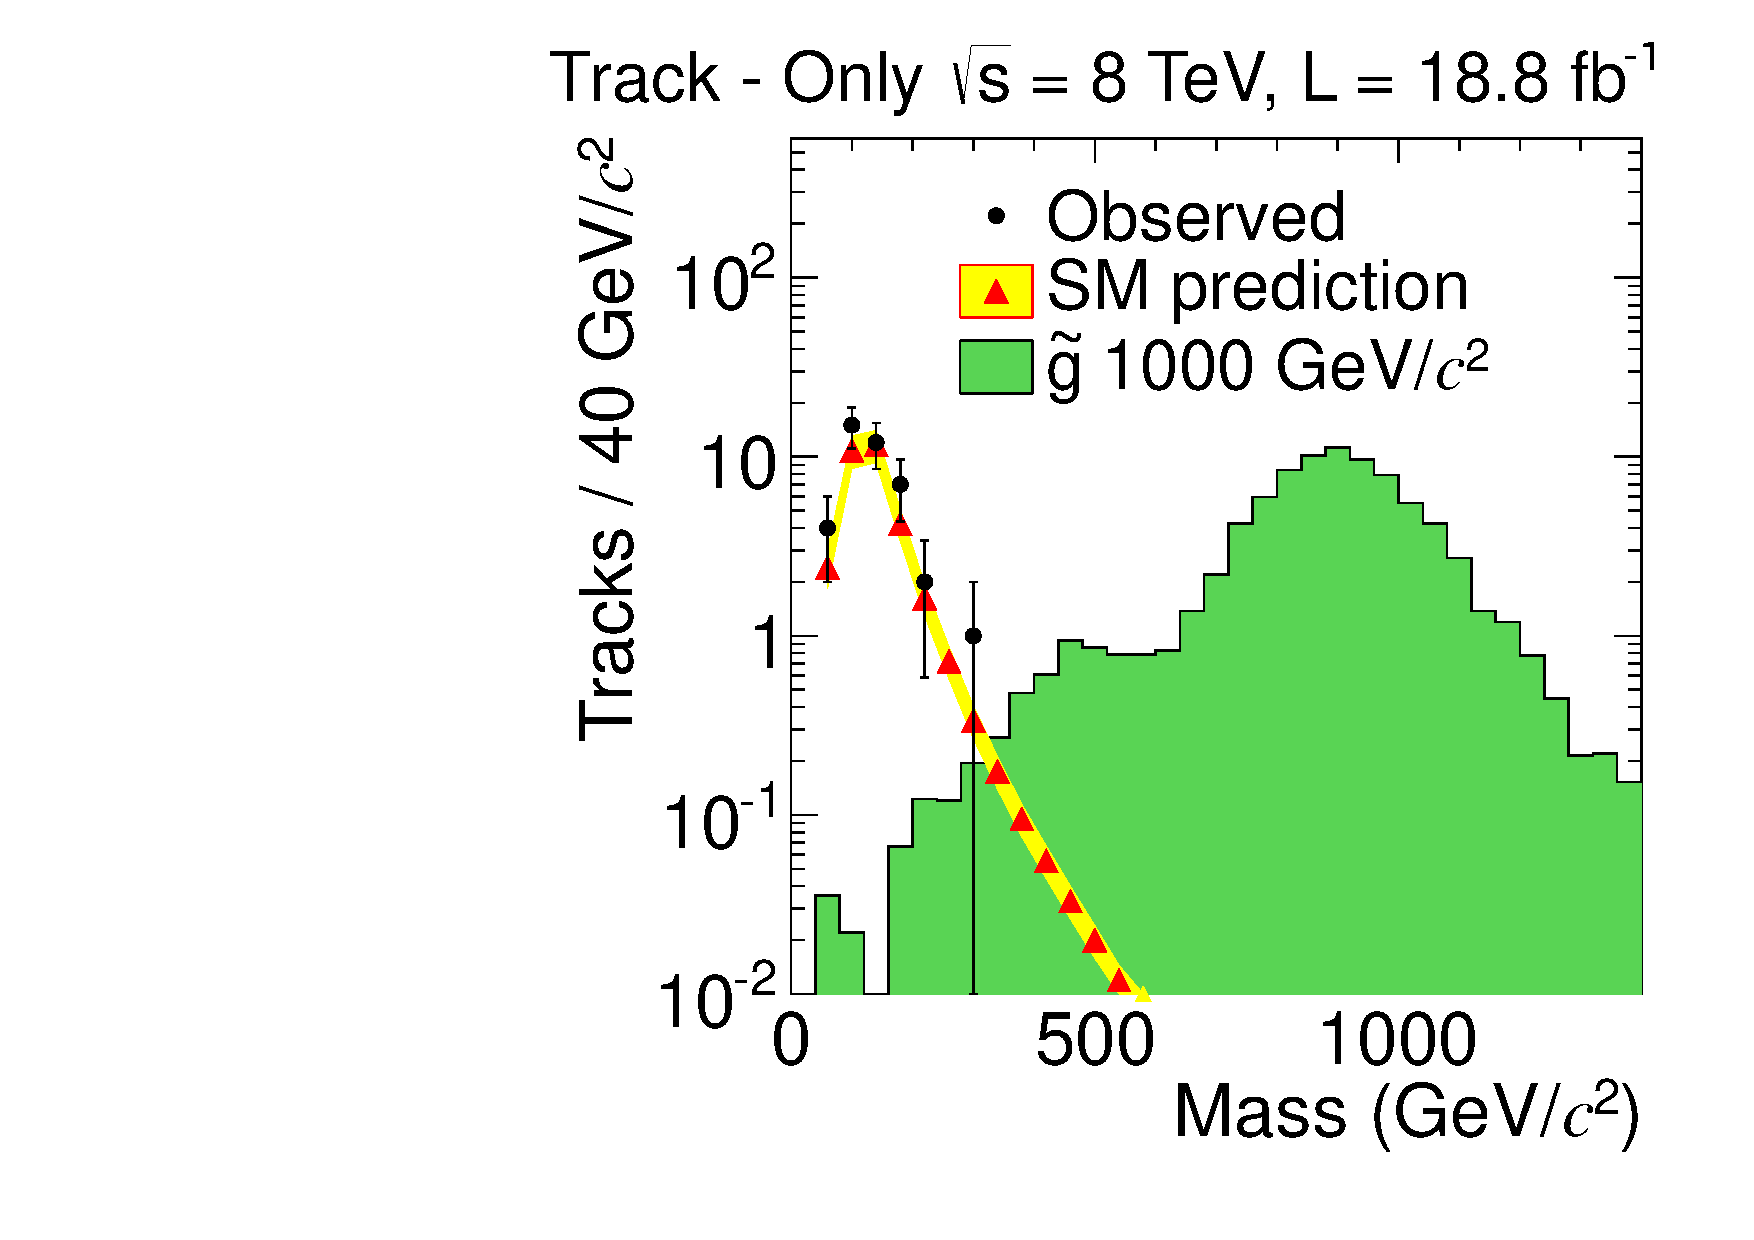
\includegraphics[clip=false, trim=0.0cm 0cm 0.0cm 0cm, width=0.48\textwidth]{figures/tkonly/RescaleNoRatio_Mass_8TeV_TightNoSMMC}
 \end{center}
 \caption[Observed and predicted mass spectrum for candidates in the signal region with the final selection thresholds in the \tktof\ and \tkonly\ analyses.]
{Observed and predicted mass spectrum for candidates in the $D$ region in the \tktof\ analysis with the tight selection.
The error bands are only statistical. Left: For the \tktof\ analysis. Right: For the \tkonly\ analysis.}
\label{fig:TightMassDistribution}
\end{figure}